\selectlanguage{english}%

\chapter{Sistemas Fuzzy} \label{capFundFuzzy}
A lógica fuzzy, ou difusa, foi introduzida originalmente por Lofti A. Zadeh, em seu artigo "Fuzzy sets and systems" \cite{zadeh}. Sua teoria diverge da lógica booleana convencional no tratamento da pertinência das variáveis, podendo assumir qualquer valor entre todos os possíveis de um intervalo. Essa abordagem é mais eficaz na descrição de alguns sistemas reais, uma vez que é praticamente impossível eliminar todas as incertezas nos modelos que os representam. Este capítulo apresenta os fundamentos desse paradigma bem como sua aplicação na modelagem, proposta por Takagi e Sugeno \cite{takagiSugeno}.

\section{Conjuntos Fuzzy}
De acordo com a teoria de conjuntos clássica, um elemento $x$ qualquer, pode pertencer ou não à um conjunto universo de discurso $U$, ou seja $x \in U$ ou $x \notin U$ . Portanto, para qualquer conjunto determinado, pode-se estar completamento dentro ou completamente fora dele.

\begin{align}
	f_u(x) : U \rightarrow \{0,1\}
	&& f_u(x) =
	\begin{cases*}
		1 & se e somente se $x \in U$ \\
		0 & caso contrário
	\end{cases*}
	\label{eqFPertinencia}
\end{align}

Essa definição binária se encaixa bem em problemas restritos, cujo caráter dos sistemas reflita essa separação clara de estados, por exemplo a paridade ou não de uma da soma dos bits de uma mensagem binária. Conhecendo-se os valores, este resulte é ímpar ou par, indubitavelmente. No entanto, grande parte dos sistemas estudados nas teorias de controle trabalha com grandezas que não possuem limites tão claros assim, como exemplo a sensação térmica. Apesar de a temperatura ser matematicamente bem definida, existem descrições como "frio" e "quente" que não podem ser representadas com este conjunto binário, uma vez que são conceitos vagos e imprecisos.

A abordagem fuzzy aparece como uma alternativa muito capaz de tratar estes casos. Seus conjuntos são caracterizados por uma função contínua de pertinência fuzzy, que relaciona cada elemento do universo de discurso à sua conformidade no conjunto, podendo abranger todos os valores no intervalo de pertinência.

\subsection{Variáveis Linguísticas}
As variáveis linguísticas são os termos que constituem os conjuntos nebulosos. Tratam-se de traduções das variáveis reais na forma de valores linguísticos, não numéricos. Assim, seguindo com exemplo anterior, a temperatura seria a variável linguística e "quente", "frio", "muito quente" e "muito frio" alguns de seus possíveis valores linguísticos. Estes últimos são os conjuntos difusos e possuem, cada um deles, uma função de pertinência mapeando a adequação de uma determinada temperatura a sua conformidade neles.

\section{Funções de Pertinência}
\label{secFncPert}
O conceito chave de toda a abordagem fuzzy são as funções de pertinência. Em exemplo, dados os conjuntos fuzzy $U_1$, $U_2$ e $U_3$, cada qual possui sua função de pertinência $f_1(x)$, $f_2(x)$ e $f_3(x)$, para todo elemento pertencente ao universo de discurso.

\begin{align}
	f_i(x) : i \rightarrow [0,1]
	\label{eqFuncPertFuzzy}
\end{align}
Onde $f_i(x)=0$ implica que o elemento $x$ é "completamente não" $U_i$ e $f_i(x)=1$ indica que $x$ é "completamente" $U_i$. Mas, diferentemente da lógica convencional, é possível que um elemento seja 50\% pertinente à $U_1$ ($f_1(x)=0.5$), 30\%  à $U_2$ ($f_2(x)=0.3$) e 20\%  à $U_3$ ($f_3(x)=0.2$).

Apesar de operar sobre grandezas linguísticas, é importante notar que normalmente os elementos são variáveis numéricas, portanto as funções de pertinência precisam ser bem definidas no intervalo do conjunto. Os formatos mais comuns para elas são apresentados na \hyperref[figPert]{Figura \ref{figPert}} a seguir:

\begin{figure}[H]
	\centering
\begin{tabular}{ccc}
	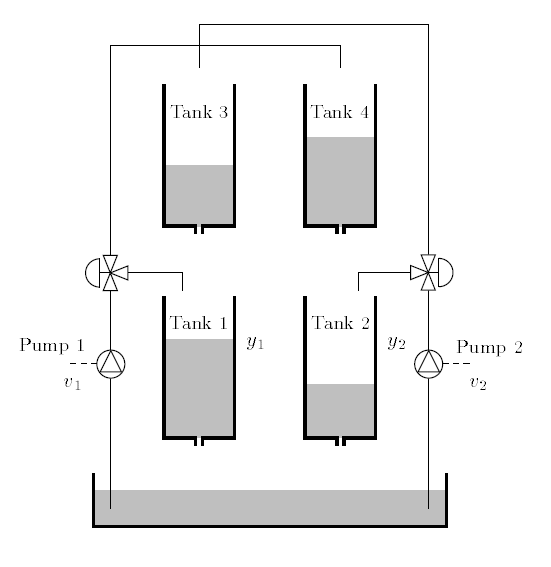
\includegraphics[width=0.3\textwidth,keepaspectratio]{img/4tank.png} &
	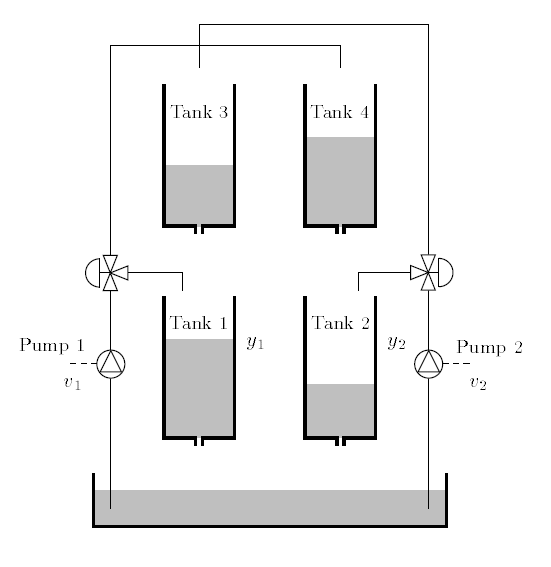
\includegraphics[width=0.3\textwidth,keepaspectratio]{img/4tank.png} &
	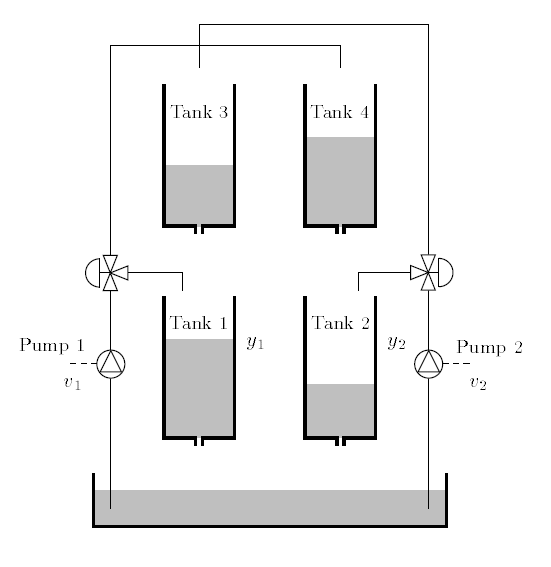
\includegraphics[width=0.3\textwidth,keepaspectratio]{img/4tank.png} \\
	(a) Triangular &
	(b) Senoidal
	(c) Trapezoidal \\
	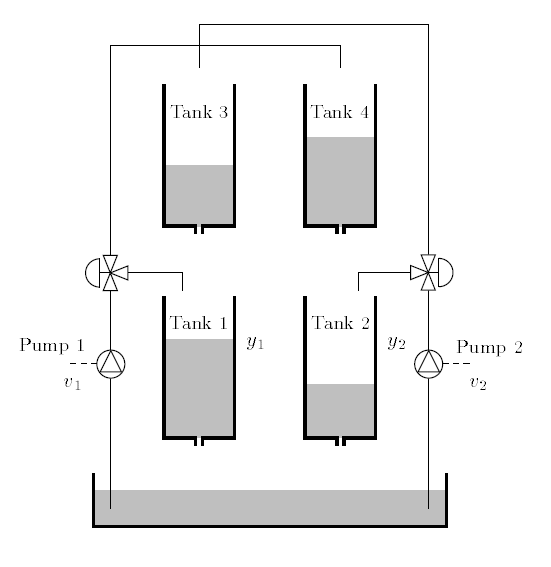
\includegraphics[width=0.3\textwidth,keepaspectratio]{img/4tank.png} &
	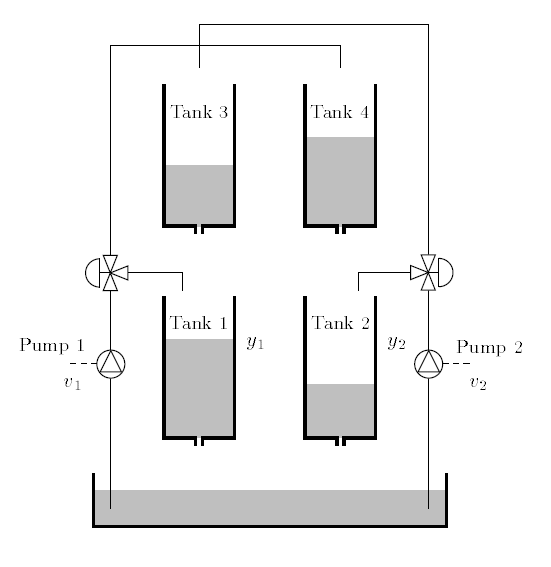
\includegraphics[width=0.3\textwidth,keepaspectratio]{img/4tank.png} &
	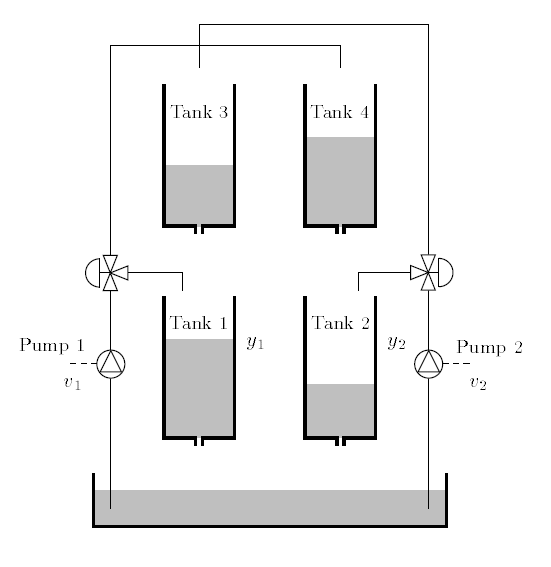
\includegraphics[width=0.3\textwidth,keepaspectratio]{img/4tank.png} \\
	(d) Gaussiana &
	(e) Sigmoide &
	(f) Quadrada
\end{tabular}
	\caption{\label{figPert}Funcões de Pertinência.}
\end{figure}

Apresenta-se a seguir os procedimentos comuns para obtenção da função de pertinência de um dado sistema, ilustrando-se com o exemplo:
\begin{itemize}
	\item \textbf{Definir a variável linguística:} "Temperatura"
	\item \textbf{Definir os conjuntos fuzzy:} \{"muito frio"\}, \{"frio"\}, \{"quente"\}, \{"muito quente"\}
	\item \textbf{Definir os limites de cada conjunto:} $[-10ºC,5ºC]$,$ [5ºC,15ºC]$, $[15ºC,30ºC]$, $[30ºC,45ºC]$ 
	\item \textbf{Definir as funções de pertinência:} Neste caso opta-se por funções triangulares, com picos nos centros dos intervalos e nulas em qualquer caso fora deles.
\end{itemize}

Os resultados do exemplo são apresentados na \jhhref{figPertEx}{Figura} a seguir:
\begin{figure}[H]
	\centering
	\begin{tabular}{cc}
		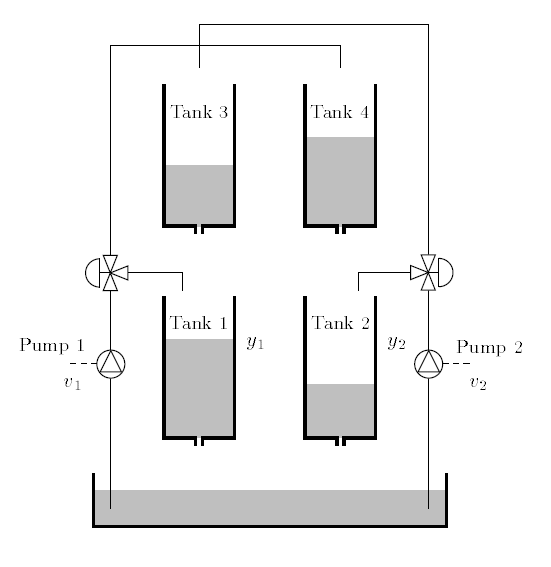
\includegraphics[width=0.3\textwidth,keepaspectratio]{img/4tank.png} &
		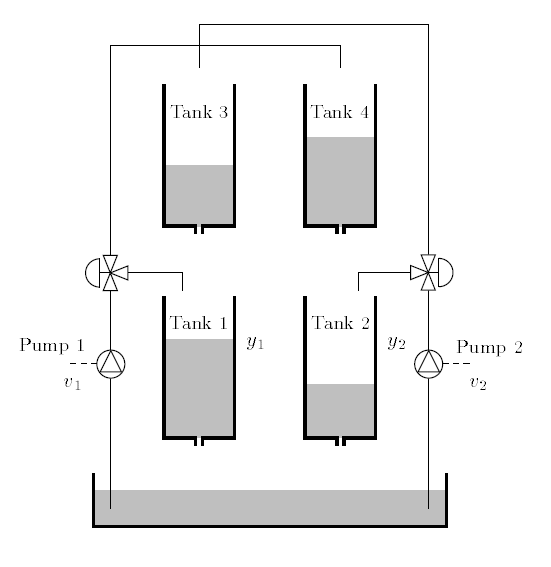
\includegraphics[width=0.3\textwidth,keepaspectratio]{img/4tank.png} \\
		(a) Pertinência do conjunto "muito frio" &
		(b) Pertinência do conjunto "frio" \\
		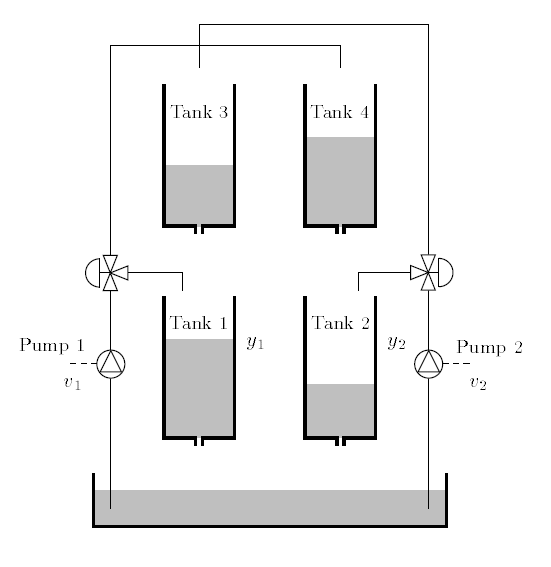
\includegraphics[width=0.3\textwidth,keepaspectratio]{img/4tank.png} &
		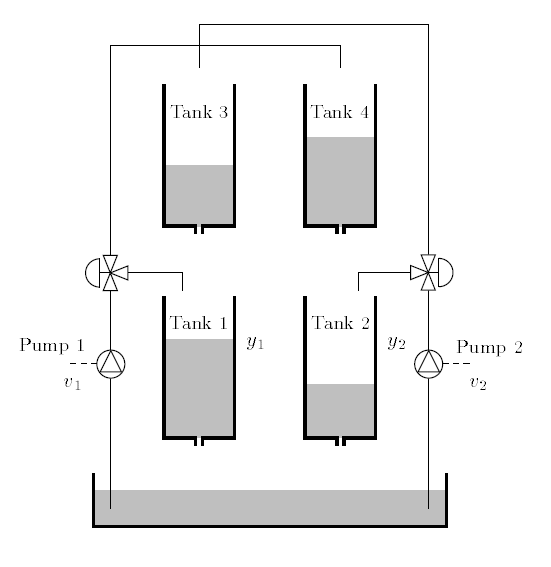
\includegraphics[width=0.3\textwidth,keepaspectratio]{img/4tank.png} \\
		(c) Pertinência do conjunto "quente" &
		(d) Pertinência do conjunto "muito quente"
	\end{tabular}
	\caption{\label{figPertEx} Funções de Pertinência.}
\end{figure}	

A \jhhref{tabPertEx}{Tabela} a seguir apresenta os graus de pertinência de várias amostras a cada conjunto:

\begin{table}[!ht]
	\caption{Tabela de Exemplos}
	\label{tabPertEx}
	\small
	\centering
	\scalebox{1}{
		\begin{tabular}{|c|c|c|c|c|}
			\hline
			Temperatura & Muito Frio & Frio & Quente & Muito Quente \\
			\hline
			0 & 0 & 0 & 0 & 0 \\
			\hline
			0 & 0 & 0 & 0 & 0 \\
			\hline
			0 & 0 & 0 & 0 & 0 \\
			\hline
			0 & 0 & 0 & 0 & 0 \\
			\hline
			0 & 0 & 0 & 0 & 0 \\
			\hline
			0 & 0 & 0 & 0 & 0 \\
			\hline
			0 & 0 & 0 & 0 & 0 \\
			\hline
			0 & 0 & 0 & 0 & 0 \\
			\hline
		\end{tabular}
	}
\end{table}

É importante notar que a soma final dos valores de todas as pertinências de um elemento precisa ser 1, para que haja coerência entre o modelo e o real.

\section{Aplicação}
A aplicação da lógica fuzzy na teoria de controle se dá através da utilização de regras que definem o modelo final baseando-se no grau de pertinência do estado do sistema a cada um dos conjuntos difusos. 

De maneira similar à tradicional, a lógica fuzzy baseia-se no paradigma de implicações, ou \textit{modus ponens}. Esta linha de raciocínio é organizada em regras que implicam em conclusões a partir da autenticidade de premissas. O \jhhref{eqRegrasEx}{exemplo} a seguir ilustra:

\begin{align} \label{eqRegrasEx}
\begin{cases}
	\text{(1) Se está  chovendo então é perigoso dirigir}\\
	\text{(2) Está chovendo }\\
	\text{(3) É perigoso dirigir}
\end{cases}		
\end{align}

A afirmação (1) é chamada de regra de implicação, ou regra Se-Então, e é ela quem rege o comportamento da conclusão (3) de acordo com a premissa (2). Ou seja, sempre que (2) é verdadeira, (3) também será.

\subsection{Regras Se-Então}
Como visto no \jhhref{eqRegrasEx}{exemplo} as regras Se-Então são parte das premissas que definem os resultados das afirmações. Uma vez que as funções de pertinência fuzzy assumem diferentes níveis de verdade, não binários, então a autenticidade de afirmações envolvendo-as também assumirá diferentes graus de verdade. Assim, ao contrário da lógica clássica onde há ou não ativação de uma determinada regra, em lógica difusa toda regra está ativada em determinado grau. Exemplifica-se a seguir:

\begin{align} \label{eqRegraDef}
\text{Regra: }
\begin{cases}
	\text{SE: X pertence a A} \\
	\text{ENTÃO: Y pertence a B}
\end{cases}		
\end{align}

O grau de ativação da Regra na \jhhref{eqRegraDef}{equação} é definido a partir da pertinência do elemento $X$ em $A$. A conclusão $Y$ será definida de forma a cumprir pertinência semelhante ao conjunto $B$. Caso $X$ seja 50\% A, a saída $Y$ deverá ser 50\% B.

Prosseguindo o exemplo inicial, pode-se utilizar a temperatura de uma sala para controlar a potência ativa de um ar condicionado.  Seguindo os procedimentos descritos, define-se uma nova variável linguística: "Potência" e seus conjuntos fuzzy: \{"muito fraca", "fraca", "forte", "muito forte"\}. Chamando "T" a temperatura atual e "P" a potência, uma forma simples de projeto poderia ser:

\begin{align*}
\text{Regra 1: }
	&\begin{cases}
		\text{SE: T pertence a "muito baixa" } \\
		\text{ENTÃO: P pertence a "muito fraca"}
	\end{cases}		\\
\text{Regra 2: }
	&\begin{cases}
		\text{SE: T pertence a "baixa"} \\
		\text{ENTÃO: P pertence a "fraca"}
	\end{cases}		\\
\text{Regra 3: }
	&\begin{cases}
		\text{SE: T pertence a "alta"} \\
		\text{ENTÃO: P pertence a "forte"}
	\end{cases}		\\
\text{Regra 4: }
	&\begin{cases}
		\text{SE: T pertence a "muito alta"} \\
		\text{ENTÃO: P pertence a "muito forte"}
	\end{cases}		
\end{align*}

\section{Modelo Fuzzy Takagi-Sugeno} \label{secTakSug}
Os trabalhos de Takagi, Sugeno \cite{takagiSugeno} e Kang \cite{kang} introduziram e desenvolveram a aplicação da lógica difusa em sistemas dinâmicos. Neles é demonstrada a capacidade dos modelos fuzzy (aqui os trataremos por Takagi-Sugeno) de representarem, de forma tão aproximada quanto se queira, qualquer sistema dinâmico (respeito condições de domínio). 

Suponha-se um sistema dinâmico qualquer a seguir:
\begin{align*}
	\dot{x(t)} &= f(x(t)) + g(u(t)) \\
	y(t) &= h(x(t))
\end{align*}

Linearizando o obteria-se o seguinte modelo em espaço de estados:
\begin{align*}
	\dot{x(t)} &= Ax(t) + Bu(t) \\
	y(t) &= Cx(t)
\end{align*}

As regras fuzzy seriam então:


\begin{align} \label{eqRegraIGeral}
	\textbf{Regra i:}
	\begin{cases}
		&\textbf{SE:} \text{ $c_1(t)$ é $M_{1i}$ e $c_2(t)$ é $M_{2i}$ e ... e $c_n(t)$ e $M_{ni}$,} \\
		&\textbf{ENTÃO}:
		\begin{cases}
			\dot{x}(t) = A_i \Delta x(t) + B_i \Delta u(t),\\
			y(t) = C_ix(t)
		\end{cases}
	\end{cases}
\end{align}

\begin{align}
	c(t) = [c_1(t) \ \ c_2(t) \ \ c_3(t) \ \ ... \ \ c_n(t)]
\end{align}
	
\begin{align}
	\begin{cases}
		\dot{x}(t) = \frac{\sum_{i=1}^{4}  w_i(c(t))(A_i \Delta x(t) +  B_i \Delta u(t))}{\sum_{i=1}^{4} w_i(c(t))} \vspace{0.5cm}\\
		y(t) = \frac{\sum_{i=1}^{4}  w_i(c(t)) C_i \Delta x(t)}{\sum_{i=1}^{4} w_i(c(t))}
	\end{cases}
\end{align}

\selectlanguage{brazil}%

